\documentclass{beamer}
%\documentclass[compressed]{beamer}
\mode<presentation>
%\usepackage{footnote}

\usetheme{Warsaw}
\useinnertheme{rectangles}
\usecolortheme{orchid}
\useoutertheme[subsection=false]{smoothbars}



\definecolor{beamer@blendedblue}{RGB}{6,105,10}

\definecolor{header_footer_color}{RGB}{2,43,3}
\setbeamercolor*{palette quaternary}{use=structure,fg=white,bg=header_footer_color}
\setbeamercolor{footlinecolor}{fg=white,bg=header_footer_color}

\beamertemplatenavigationsymbolsempty

\setbeamertemplate{footline}{
\begin{beamercolorbox}[sep=2pt,wd=\paperwidth,leftskip=0.5cm,rightskip=0.5cm]{footlinecolor}
\centering \bf{\hspace{50pt} CS300A : Techincal Paper Review
 \hfill \insertframenumber}
\end{beamercolorbox}
}

\usepackage{hyperref}

\usepackage{float}
\usepackage{fancyhdr}
\usepackage[bottom,norule]{footmisc}
\usepackage{subfigure}
\usepackage{setspace}
\usepackage{color,colortbl}
\usepackage{graphicx}
\usepackage{xcolor}         
\usepackage{color}
\usepackage{multimedia}
\usepackage{mathtools}



\definecolor{rowcolor}{rgb}{0.65,0.9,0.9}
\definecolor{blockcolor}{RGB}{157,227,222}


\title{\large On Chubanov's method for Linear Programming \\ A. Basu, J. A. De Loera, M. Junod
et al }
\author{Saurav Shekhar\inst{1}}
\institute{\tiny $^1$Department of Computer Science \& Engineering, IIT Kanpur\\ 
E-mail: sshekh@iitk.ac.in
}
\date{\tiny 27 October, 2014}

\begin{document}
\setbeamercolor{block body}{bg=blockcolor} 

\frame{
	\thispagestyle{empty}		%Hiding frame number
	\titlepage
}


\frame{\setcounter{framenumber}{0}\frametitle{Contents}\tableofcontents}

\section{The Problem}

\begin{frame}
\setcounter{framenumber}{1}
\frametitle{The Problem}
Determining the feasibility of the systems of the form 
\begin{center} $Ax = b, Cx \leq d$ \end{center}
 in $\mathbb{R}^{n}$, with $A$ an $m \times n$ matrix, $C$ an $l \times n$ matrix, $b \in \mathbb{R}^{n}$ , and $d \in \mathbb{R}^{l}$ , where the elements
of $A$, $b$, $C$, and $d$ are integers, or determine if the system has no integer solutions.

This is the \emph{Linear Feasiblity Problem (LPP)}, and has been used to model transportation problems, airline scheduling, networks etc.
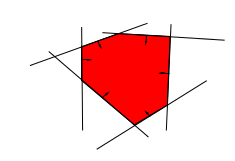
\includegraphics[width=0.4\textwidth]{fig/feasible_region.png}

\end{frame}

\section{Previous Methods}

\begin{frame}{Previous Methods}
\begin{itemize}
 \item AMS Relaxtion method (by Agmon, Motzkin and Schoenberg)
 \pause
 \item Starting from any initial point, a sequence of points is generated
 \pause
 \item If the current point $z_{i}$ is feasible we stop
 \pause
 \item Else project $z_{i}$ over the hyperplane defined by the violated constraint $c^{T}x \leq d$
 \pause
 \item If the original system is feasible, the points generated will converge to a solution.
 \pause
 \item Has been shown to take exponential time.
\end{itemize}

\pause

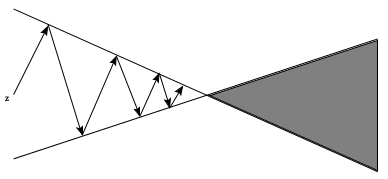
\includegraphics[width=0.7\textwidth]{fig/ams.png}

\end{frame}

\section{Algorithm}
% 
% \begin{frame}{Block Scheme}
% 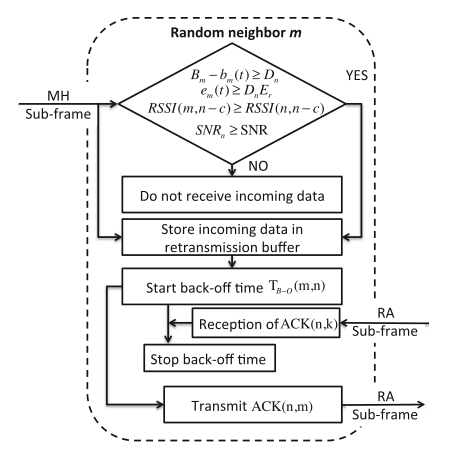
\includegraphics[width=0.7\textwidth]{fig/cs300b.png}
% \end{frame}

\begin{frame}
 \frametitle{The Chubanov Divide and Conquer algorithm}
 Given a current guess $z$, a radius $r$ and an error bound $\epsilon > 0$, the algorithm will either:
 \begin{itemize}
  \item Find an $\epsilon$ approximate solution $x^{*} \in \text{ ball }B(z, r)$ to the system, i.e some $x^{*}$ such that \\
	$Ax^{*} = b, Cx^{*} \leq d + \epsilon \bf{1}$ 
  \pause
  \item Or find an induced hyperplane $hx = \delta$ that separates $B(z, r)$ from $P$.
 \end{itemize}
\pause

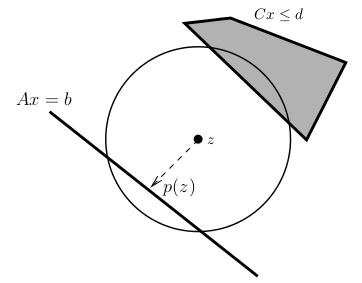
\includegraphics[width=0.7\textwidth]{fig/ball.png}

 
\end{frame}

\begin{frame}
 \frametitle{Advantages of Induced hyperplanes}
 \begin{itemize}
  \item These are new constraints derived as convex combinations of the original ones.
  \pause
  \item When $Cx \leq d$ takes the form of $\bf{0} \leq x \leq \bf{1}$, Chubanov's algorithm runs in strongly polynomial time.
 \end{itemize}
  \pause
  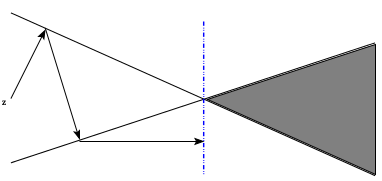
\includegraphics[width=0.7\textwidth]{fig/dc.png}
 
\end{frame}


\section{Extensions and Results}

\begin{frame}{Extensions and Results}
Theory:
\begin{itemize}
 \item Chubanov's algorithm either returns a feasible solution or determines that no feasible solution exist.
 \item We use $D\&C$ to determine the feasibility of strict LFP's. 
\end{itemize}
Practical Numerical Analysis:
\begin{itemize}
 \item Despite its theoretical advantages, Chubanov's Relaxtion method appears to be practically much slower than the original relaxation method.
\end{itemize}

\end{frame}


\begin{thebibliography}{99}
\begin{frame}[allowframebreaks]{title}
\frametitle{References}
{\scriptsize
\setbeamertemplate{bibliography item}[article]
\bibitem{}
S. Agmon ``The relaxation method for linear inequalities.'' in \emph{Canadian J. Math}, 6:382-392, 1954
\bibitem{}
S. Chubanov ``A strongly polynomial time algorithm for linear systems having a binary solution'' in \emph{Mathematical Programming} pages 1-38, 2011. 10.1007/s10107-011-0445-3
\bibitem{}
T.S. Motzkin and I. J. Schoenberg ``The relaxation method for ilnear inequalities'' in \emph{Canadian J. Math} 6:393-404, 1954
\bibitem{}
E.Tardos ``A strongly polynomial time algorithm to solve combinatorial linear programs'' in \emph{Math. of Oper. Res.}, 34(2):250-256, 1986

}
\end{frame}
\end{thebibliography}


\begin{frame}
\thispagestyle{empty}
\begin{center}
\Huge Thank You!
\end{center}
\vspace*{10pt}
\vspace*{10pt}
\vspace*{10pt}
\vspace*{10pt}
\vspace*{10pt}
\vspace*{10pt}
\vspace*{10pt}

%\blfootnote{\tiny Thanks to Sharbatanu Chatterjee the \LaTeX template}
\end{frame}

\end{document}

